\documentclass[t, 
			   13pt,				            
			   final, 				         
			   xcolor={usenames,dvipsnames}, 
			   table]{beamer}


\usepackage{amsmath}
\usepackage[brazil]{babel}
\usepackage[utf8]{inputenc}
\usepackage{booktabs}
\usepackage[alf]{abntex2cite}
\usepackage{caption}


\usepackage{todo}

% configuração do tema
\usetheme[pageofpages=de,
          bullet=square,			
          titleline=true,				
          alternativetitlepage=true,			
          titlepagelogo=imagens/logo-puc,	
          watermarkheight=70px,		
          watermarkheightmult=4	
          ]{Torino}

\setbeamertemplate{sections/subsections in toc}[square]
\setbeamertemplate{bibliography item}[default]

\usecolortheme{freewilly}

\logo{
\includegraphics[height=0.110\paperheight]{imagens/logo-puc}}

\begin{document}
	\author{Luiz Alberto Ferreira Gomes}
\title{Aplicações Web com Ruby On Rails}
\subtitle{Seminários da Computação}
\institute{Curso de Ciência da Computação}
\date{\today}

    \begin{frame}[plain]
  \titlepage
\end{frame}
    \AtBeginSection[]
{
  \begin{frame}{Agenda}
    \tableofcontents[currentsection]
  \end{frame}
}
  
   	\section{Apresentaço do Curso}

%%-------------------------------------------------------------------------------------- Início
\begin{frame}[fragile,t]{Apresentação do Curso}
  \begin{itemize}
    \item Este curso tem como objetivo explorar o \alert{desenvolvimento de aplicações web} considerando 
      \alert{padrões de projetos} fundamentais e filosofias associadas a \alert{arquiteturas modernas} de aplicações web
      , juntamente com os seus principais componentes.
    \item Ao final deste curso, espera-se que o aluno seja capaz de:
    \begin{itemize}
      \item projetar, desenvolver e publicar uma aplicação web;
      \item entender os principais \alert{componentes} da arquitetura web apps e como eles se interagem;
      \item utilizar a plataforma Ruby on Rails;
      \item compreender melhor as \alert{práticas} modernas de engenharia de software.
    \end{itemize}
  \end{itemize}
\end{frame}
%%-------------------------------------------------------------------------------------- Início
\begin{frame}[fragile,t]{Conteúdo Programático}
    \begin{center}
      \begin{tabular}{| p{2cm} | p{8cm} |}
	\hline
	\textbf{Data} & \textbf{Módulo} \\ \hline
	18/09 & Introdução e Conceituação \\ \hline
	25/09 & Ruby on Rails \\ \hline
	02/10 & Interação com Banco de Dados \\ \hline
	09/10 & A Linguagem de Programação Ruby \\ \hline
	16/10 & A Linguagem de Programação Ruby \\ \hline
	23/10 & Middleware \\ \hline
	30/10 & Interface com o Usuário \\ \hline
	\hline
      \end{tabular}
    \end{center}  
\end{frame}
%%-------------------------------------------------------------------------------------- Início
\begin{frame}[fragile,t]{Histórico}
  \begin{figure}[h!]
    \centering
    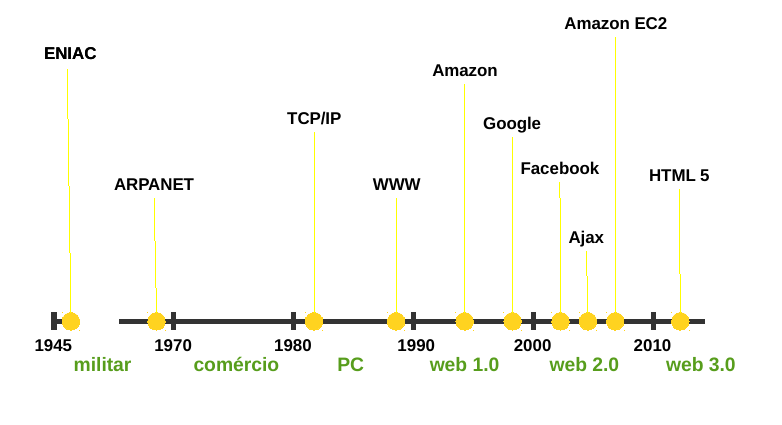
\includegraphics[width=0.95\textwidth]{imagens/historico.png}
  \end{figure} 
\end{frame}
%%-------------------------------------------------------------------------------------- Início
\begin{frame}[fragile,t]{Web 1.0, 2.0 e 3.0}
  \begin{itemize}
    \item \alert{Web 1.0} : páginas estáticas e primeiros modelos de negócios.
    \item \alert{Web 2.0} : interactividade(Ajax), redes sociais e comércio eletrônico.
    \item \alert{Web 3.0} : 'Web Inteligente', interpretação da informação auxiliada por máquina 
    \begin{itemize}
      \item exemplo: sistemas de recomendação.
    \end{itemize}
    \item Base tecnológica da Web 2.0 e 3.0.
    \begin{itemize}
      \item javascript, xml, json(ajax).
      \item interoperabilidade via Web Services.
      \item infraestrutura via modelos de \alert{computação em nuvem} (IAAS, PAAS e SAAS)
      \item aplicações móveis
    \end{itemize}
  \end{itemize}
\end{frame}
%%-------------------------------------------------------------------------------------- Início
\begin{frame}[allowframebreaks, fragile,t]{Modelos de Computação em Nuvem}
  
  \begin{itemize}

    \item \alert{IAAS (Infraestructure As A Service)} : fornece a insfraestrutura computacional
      física ou máquinas virtuais e outros recursos discos, firewalls, endereços IP e etc.
    \begin{itemize}
     \item exemplos: Amazon EC2, Windows Azure, Google Compute Engine.
    \end{itemize}
    
    \item \alert{PAAS (Platform as a Service)} : fornece plataformas computacionais que tipicamente incluem sistemas operacionais,
      ambientes para execução de programas, bancos de dados, servidores web e etc.
    \begin{itemize}
     \item exemplos: AWS Elastic Beanstalk, Windows Azure, Heroku e Google App Engine
    \end{itemize}

    \item \alert{SAAS (Software as a Service)} : fornece acesso sob demanda às aplicações de software, sem que o usuário
      tem que se preocupar com sua instalação, configuração e execução.
    \begin{itemize}
     \item exemplos: Google Apps e Microsoft 365.
    \end{itemize}
 
  \end{itemize}
 
\end{frame}
   	\section{Aplicação Web}
%%-------------------------------------------------------------------------------------- Início

%%-------------------------------------------------------------------------------------- Início
\begin{frame}[allowframebreaks, fragile,t]{Aplicação Web}
  \begin{exampleblock}{Definição(Aplicação Web)}
    Uma \alert{aplicação web} é aquela que acessada pelos usuários por meio de uma \alert{rede de computadores}, utiliza
    um \alert{navegador} (em inglês: \textit{browser}); e consiste de uma coleção de \alert{\textit{scripts}} no cliente e 
    no servidor, páginas \alert{HTML} e outros recursos que podem estar espalhados por vários servidores. Ele é 
    acessada pelos usuários via \alert{um endereço} que faz referência a um servidor web (por exemplo: www.inf.pucpcaldadas.br).
  \end{exampleblock}
  
  \begin{itemize}
    \item Exemplos: webmail, lojas virtuais, homebanking, wikis, blogs e etc.
  \end{itemize}
  
\framebreak

  \begin{itemize}
    \item Há um pouco mais do que isso:
    \begin{itemize}
      \item Rede de Computadores:
      \begin{itemize}
        \item a \alert{Internet}, um sistema global de redes de computadores interconectadas.
        \item utiliza o conjunto de protocolos TCP/IP.
      \end{itemize}
      \item Web (World Wide Web):
      \begin{itemize}
	\item um sistema de documentos (em inglês: \textit{web pages}) \alert{vinculados} que são acessados através 
	  da Internet via protocolo HTTP.
	\item Web pages contêm documentos \alert{hypermedia}: textos, gráficos, imagens, vídeos e outros recursos multimídia, juntamente com \textit{hiperlinks} para outras páginas
	\item \alert{Hiperlinks} formam a \alert{estrutura básica} da Web.
	\item A estrutura da Web é a que a torna \alert{útil} e de \alert{valor}.
      \end{itemize}
    \end{itemize}
    \item \underline{Vantagens}:
    \begin{itemize}
      \item \alert{Conveniência} pela utilização um web browser como cliente. 
      \item \alert{Compatibilidade} inerente entre plataformas.
      \item Habilidade de \alert{atualizar} e \alert{manter} as aplicações web sem instalação e distribuição de software
        em vários clientes em potencial.
      \item \alert{Redução} dos custos de TI.
    \end{itemize}
    \item \alert{Desvantagens}:
    \begin{itemize}
      \item Interfaces com usuário ainda \alert{não são tão boas} quanto as das aplicações tradicionais.
      \item Maior risco de \alert{comprometimento} da \alert{privacidade} e \alert{segurança dos dados}.
      \item Mais \alert{difícil} de \alert{desenvolver} e \alert{depurar} do que uma aplicação tradicional, pois 
        existem mais partes a se considerar.
    \end{itemize}
  \end{itemize}
\end{frame}
%%-------------------------------------------------------------------------------------- Início
   	%\section{Arquiteturas de WebApps?}
%%-------------------------------------------------------------------------------------- Início
\begin{frame}[allowframebreaks, fragile,t]{Arquiteturas de Aplicações Web}
  \begin{itemize}
    \item As aplicações \alert{web modernas} envolvem uma quantidade significativa de \alert{complexidade}.
    \begin{itemize}
      \item especialmente no lado do servidor.
    \end{itemize}
    \item Uma típica aplicação web envolve \alert{inúmeros protocolos}, \alert{linguagens de programação} e 
      \alert{tecnologias} que compõem a pilha de tecnologia web. 
    \item Desenvolver, manter e ampliar uma aplicação web complexa é \alert{difícil}.
    \begin{itemize}
      \item mas, construindo-o usando uma \alert{base de princípios de sólidos de projeto} pode-se simplificar 
      cada uma dessas tarefas. 
    \end{itemize}
    \item Engenheiros de software usam \alert{abstrações} para lidar com este tipo de complexidade.
    \begin{itemize}
      \item \textit{Design patterns} fornecem abstrações úteis para sistemas orientados a objetos.
    \end{itemize} 
  \end{itemize}
\end{frame}
%%-------------------------------------------------------------------------------------- Início
\begin{frame}[allowframebreaks, fragile,t]{Design Patterns}
  \begin{exampleblock}{Definição (Design Patterns)}
    Um padrão de projeto é uma descrição da \alert{colaboração de objetos} que interagem para resolver 
    um problema de software em geral dentro de um contexto particular.
  \end{exampleblock}
  \begin{itemize}
    \item Um design pattern é um \alert{modelo abstrato} que pode ser aplicado recorrentemente.
    \item A idéia é aplicar padrões de projeto, a fim de \alert{resolver problemas específicos} que ocorrem 
      durante a construção de sistemas reais.
    \item Os padrões de projeto fornecem uma maneira de \alert{comunicar} as soluções em um projeto, ou seja, 
      é a terminologia que engenheiros de software usam para falar sobre projetos.
  \end{itemize}
\end{frame}
%%-------------------------------------------------------------------------------------- Início
\begin{frame}[allowframebreaks, fragile,t]{Modelo Cliente-Servidor}
	\begin{itemize}
		\item A arquitetura \alert{cliente-servidor} é a arquitetura mais básica para descrever a cooperação
		entre os componentes de uma aplicação web.
		\item A arquitetura cliente-servidor pode ser subdividia em:
		\begin{itemize}
			\item \alert{servidor} que "escuta" por requisições e fornece os serviços ou recursos de acordo com 
			cada  uma.
			\item \alert{cliente} que estabelece a conexão com o servidor para requisitar serviços ou recursos.
		\end{itemize}
		\item Existe um protocolo \alert{request/response} associado com qualquer arquitetura cliente-servidor.
	\end{itemize}
	\begin{figure}[h!]
		\centering
		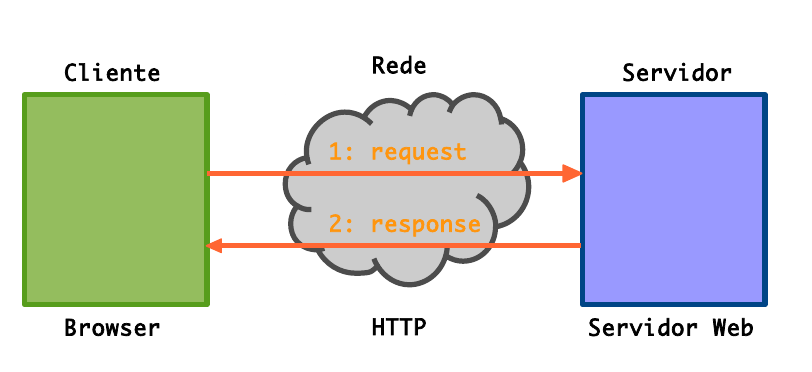
\includegraphics[width=0.90\textwidth]{imagens/cliente-servidor-1.png}
		\caption{Arquitetura cliente servidor.}
	\end{figure} 
	
\framebreak
  \begin{itemize}
    \item É sem dúvida é o padrão de projeto de arquitetura mais conhecido
    \item O ponto chave de uma arquitetura cliente-servidor é \alert{distribuir} os componentes de uma 
      aplicação entre o cliente o servidor de alguma forma. 
    \begin{itemize}
        \item o servidor realiza as tarefas, consultas e transações
        \item o cliente fica com uma responsabilidade menor: a de receber informações
    \end{itemize} 
    \item A fim de construir aplicações web complexas, vários design patterns ajudam a \alert{organizar} como peças 
      são dispostas dentro da arquitetura cliente-servidor.
  \end{itemize}
\end{frame}
%%-------------------------------------------------------------------------------------- Início
\begin{frame}[allowframebreaks, fragile,t]{Arquitetura N-Tier}
  \begin{exampleblock}{Definição (Arquitetura N-Tier)}
    A arquitetura n-tier é um \textit{design pattern} muito útil que estrutura o modelo cliente-servidor.
  \end{exampleblock}
  \begin{itemize}
    \item Este padrão de projeto é baseado no conceito de \alert{quebrar} um sistema em partes diferentes ou 
      camadas que podem ser separados fisicamente:
    \begin{itemize}
      \item cada camada é responsável por fornecer uma \alert{funcionalidade específica} ou coesa. 
      \item uma camada apenas interage com as \alert{camadas adjacentes} a ela por meio de uma 
	\alert{estrutura} bem definida por meio de \alert{interfaces}.
    \end{itemize}
  \end{itemize}
  \begin{exampleblock}{Exemplos (Arquitetura 2-Tier)}
    \begin{itemize}
      \item Servidores de impressão
      \item Aplicações web antigas:
      \begin{itemize}
        \item Interface com o usuário (navegador) residia no cliente (thin). 
        \item Servidor fornecia as páginas estáticas (HTML). 
        \item Interface entre os dois via \textit{Hypertext Transfer Protocol} (HTTP).
      \end{itemize}
    \end{itemize}
  \end{exampleblock}
  \begin{itemize}
    \item Camadas \alert{adicionais} aparecem quando a \alert{funcionalidade} do aplicativo é ainda 
      \alert{mais dividida}.
    \item Quais são as vantagens de um tal projeto? 
    \begin{itemize}
      \item A abstração fornece um meio para \alert{gerenciar} a complexidade. 
      \item Camadas podem ser atualizados ou substituídos de forma \alert{independente} 
	a medida que os requisitos ou tecnologia.
      \begin{itemize}
       \item  a nova só precisa usar as \alert{mesmas interfaces} que a antiga utilizada. 
      \end{itemize}
      \item Ele fornece um \alert{equilíbrio} entre inovação e padronização. 
      \item Sistemas tendem a ser muito mais \alert{fáceis} de construir, manter e atualizar.
    \end{itemize}
  \end{itemize}

\end{frame}
%%-------------------------------------------------------------------------------------- Início
\begin{frame}[allowframebreaks, fragile,t]{Arquitetura 3-Tiers}
  \begin{itemize}
    \item Uma das mais comuns é a arquitetura em 3 camadas: 
    \begin{itemize}
      \item Apresentação
      \begin{itemize}
       \item a interface com o usuário. 
      \end{itemize}     
      \item Aplicação (lógica)
      \begin{itemize}
	\item recupera modifica e$/$ou exclui dados na camada de dados, e envia os resultados do processamento
	para a camada de apresentação. 
      \end{itemize}
      \item Camada de dados
      \begin{itemize}
       \item a fonte dos dados associados ao aplicativo.
      \end{itemize}
    \end{itemize}
 
    \item As aplicações web modernas frequentemente são construídas \alert{utilizando} uma arquitetura em 3 camadas: 
    \begin{itemize}
      \item Apresentação
      \begin{itemize}
	\item o navegador web do usuário. 
      \end{itemize}

      \item Aplicação (lógica) 
      \begin{itemize}     
	\item o servidor web e lógica associada com \alert{geração} de conteúdo web dinâmico.
	\item por exemplo, a coleta e formatação do resultados de uma pesquisa. 
      \end{itemize}
      
      \item Camada de dados
      \begin{itemize}    
	\item um banco de dados.
      \end{itemize}
      
    \end{itemize}
    
  \end{itemize}
\end{frame}
%%-------------------------------------------------------------------------------------- Início
%\begin{frame}[allowframebreaks, fragile,t]{Arquitetura 6-Tiers para Aplicações Web }
%  \begin{itemize}
%    \item A camada de aplicação é frequentemente subdividida em dois níveis:
%    \begin{itemize} 
%      \item Camada de lógica de negócios
%      \begin{itemize}
%	\item modelos os \alert{objetos de negócios} associados ao aplicativo, por exemplo, contas, estoques, etc.
%	\item captura as regras de negócio associadas a esses objetos.     
%       \end{itemize}      
%      \item Camada de acesso a dados
%      \begin{itemize}
%	\item responsável por acessar os dados e passá-los para a camada de lógica de negócios.
%	\item por exemplo, saldos de contas, transações, etc.
%      \end{itemize}
%    \end{itemize}
%    \item A camada de apresentação é muitas vezes subdividida em dois níveis: 
%    \begin{itemize}
%      \item Camada de clientes
%      \begin{itemize}
%	\item os componentes da interface do usuário do lado do cliente.
%      \end{itemize}
%      
%      \item Apresentação camada de lógica
%      \begin{itemize}
%       \item scripts do lado do servidor para a geração de páginas web. 
%      \end{itemize}
%
%    \end{itemize}
%    \item Finalmente, o servidor web é muitas vezes separados em sua própria camada da Web e o
%    servidor de banco de dados na sua camada de dados.
%  \end{itemize}
%  
%  \begin{figure}[h!]
%    \centering
%    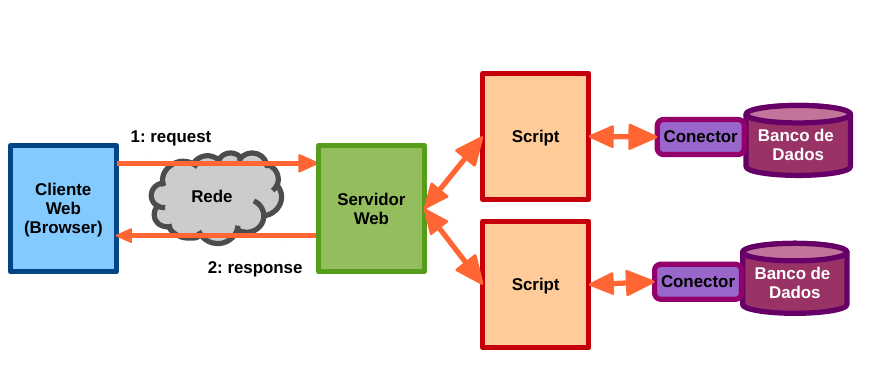
\includegraphics[width=0.95\textwidth]{imagens/cliente-servidor-2.png}
%    \caption{Arquitetura em 6 Camadas.}
%  \end{figure}
%  
%\end{frame}
%%%-------------------------------------------------------------------------------------- Início
   	%%-------------------------------------------------------------------------------------- Início
\begin{frame}[fragile,t]{Para Saber Mais}
  \begin{itemize}
    \item \url{https://www.ruby-lang.org/en/}
    \begin{itemize}
     \item referência oficial da linguagem Ruby onde a toda a sua documentação está disponível
	para ser consultada.
    \end{itemize}

    \item \url{http://rubyonrails.org/}
    \begin{itemize}
     \item referência oficial do framework Rails onde a toda a sua documentação está disponível
	para ser consultada.
    \end{itemize}
    
    \item \url{http://www.codecademy.com/pt/tracks/ruby}
    \begin{itemize}
     \item interessante curso iterativo em portugês sobre a linguagem Ruby.
    \end{itemize}

  \end{itemize}
  
  
\end{frame}
	\section{Por Dentro do Rails}

\begin{frame}[allowframebreaks, t, fragile]{Por Dentro do Rails}
	\begin{itemize}
		\item Ruby on Rails (Rails) é framework para o desenvolvimento de aplicações web
		\item Construído utilizando a linguagem Ruby
		\item 100\% open-source - MIT license
		\item Fornece a pilha completa para Web apps
		\item Lançado em 2004 e continua evoluindo rapidamente
		\item Algumas empresas que utilizam Rails: Twitter, Hulu, GitHub, Yellow Pages e etc
	\end{itemize}
\framebreak
	\begin{itemize}
		\item Rails é uma \alert{gem} Ruby (gem é um pacote Ruby)
		\item Rails fornece uma extenso conjunto de geradores de código e scripts de automação de testes
		\item Um conjunto de ferramentas adicionais são fornecidos como parte do ecossistema Rails:
		\begin{itemize}
			\item \alert{Rake} - utilitário similar ao \textbf{make do Unix} para criar e migrar bancos de dados, limpar sessões de uma Web app
			\item \alert{WEBrick} - servidor web de desenvolvimento para execução de aplicações Rails
			\item \alert{SQLite} - um servidor de banco de dados simples pré-instalado como o Rails
			\item \alert{Rack Middleware} - interface padronizado para interação entre um servidor web e uma Web App
		\end{itemize}
	\end{itemize}
\end{frame}

\begin{frame}[t, fragile]{Model-View-Controller}
	\begin{itemize}
		\item O framework Rails é contruído em cima do Design Pattern Model View Controller(MVC):
	\end{itemize}
	\begin{figure}[h!]
		\centering
		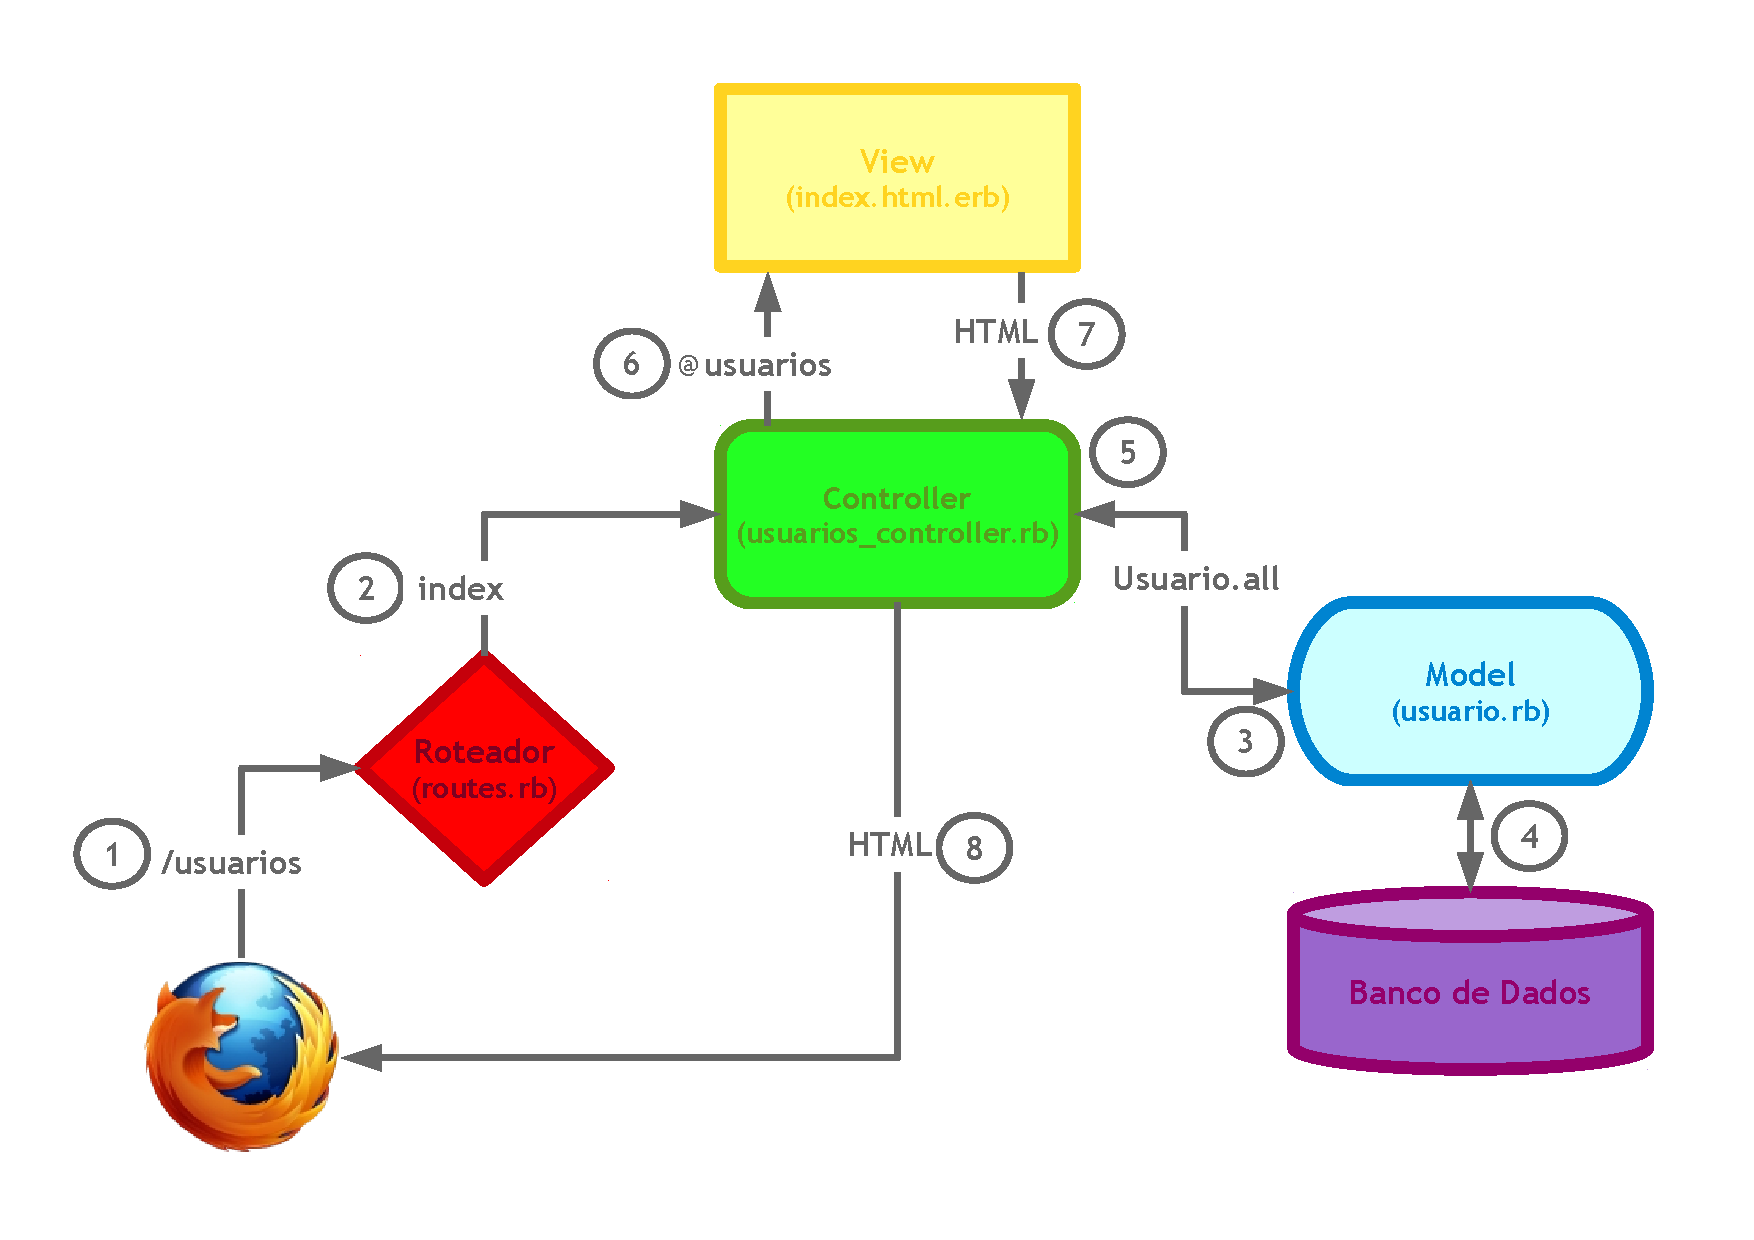
\includegraphics[width=0.70\textwidth]{imagens/mvc-1.pdf}
	\end{figure}
\end{frame}
%    \include{MVC}
%    \include{Artigos}
%    \include{Artigo1}
%    \include{Artigo1-Objetivos}
%    \include{Artigo1-Metodologia}
%    \include{Artigo1-Resultados}
%    \include{Artigo2}
%    \include{Artigo2-Objetivos}
%    \include{Artigo2-Metodologia}
%    \include{Artigo2-Resultados}
%    \include{Artigo3}
%    \include{Artigo3-Objetivos}
%    \include{Artigo3-Metodologia}
%    \include{Artigo3-Resultados}
%    \include{Consolidacao}
%    \include{Discussao}
%    \include{Conclusoes}
    \nocite{Cortes2001}
\nocite{Broy2006}
\nocite{Coleman1994}
\nocite{Bennett2000}
\nocite{Vale2015}
\nocite{Sommerville2011}
\nocite{Hanafi2015}
\nocite{Bagheri2011}
\nocite{Cafeo2013}
\nocite{Gomaa2005}
    \include{Bibliografia}
\end{document}

